\documentclass{article}
\usepackage[utf8]{inputenc}
\usepackage{varioref}
\usepackage[english]{babel}
\usepackage{pdfpages}

\title{LaboOS-opdracht1: Simulatie van Scheduling Algoritmes}
\author{Piet Vanhaute \& \mbox{Pieter-Jan} Robrecht}
\date{Maart 2016}
\usepackage{natbib}
\usepackage{graphicx}

\begin{document}

%\maketitle
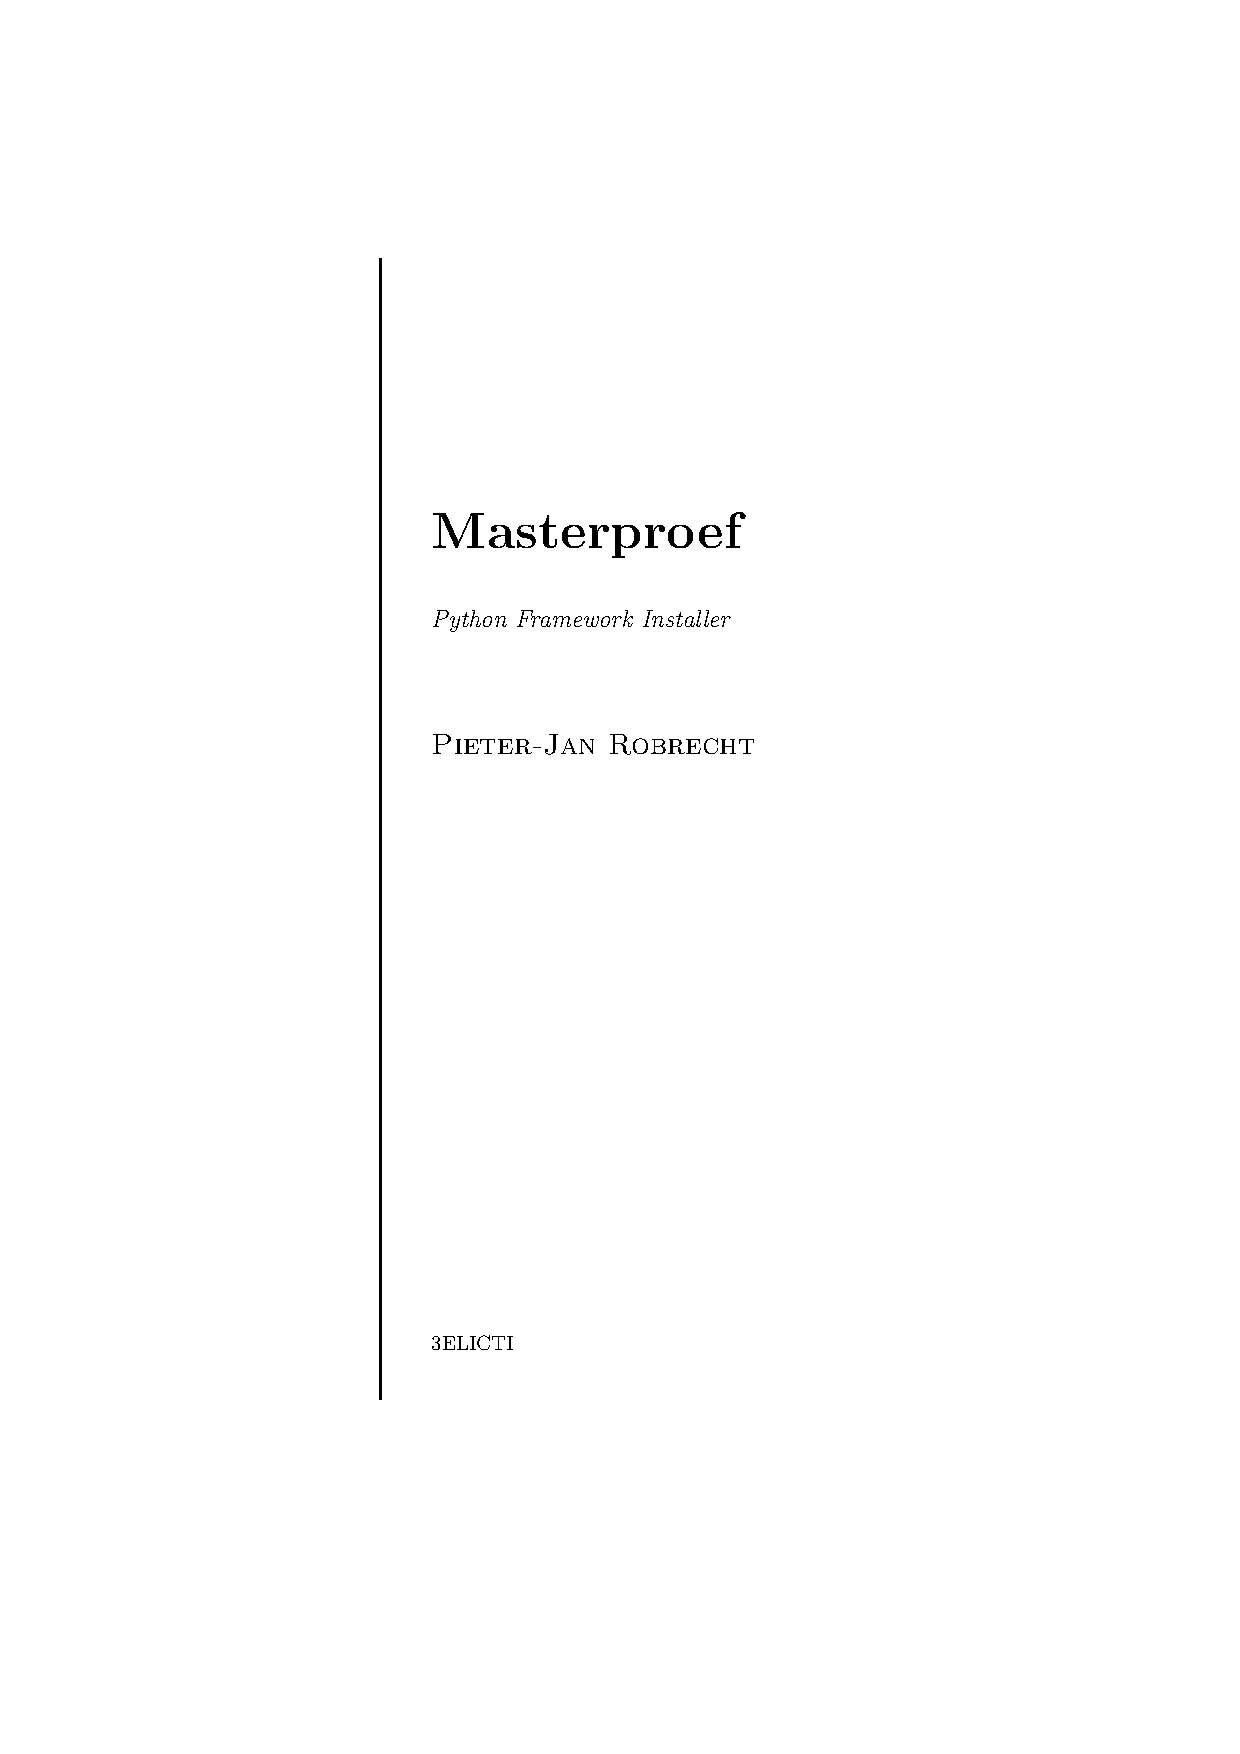
\includepdf{titel/titelpagina.pdf}

%Volgende lijn is om de titelpagina geen paginanummer te geven
\clearpage
\setcounter{page}{1}

\tableofcontents
\clearpage

\section{Abstract}
\section{Introduction}
\section{Experiments}
\section{Results}
\section{Discussion}
\section{Conclusion and future work}
\section{Acknowledgments}
\section{References}
\section{Appendix}


\end{document}